

\section{\textit{Virtual Closed-Loop Prosthesis}}

Investigating the usability of the two sensory configurations in a closed-loop scenario required these to be interfaced with a prosthetic device, which accommodated the performance of rotational and open/closed hand DoF's. However, using an actual prosthesis would result in auditory feedback being provided to the subject, though prosthetic actuation sounds, eliminating the interest of solely exploring the impact sensory feedback. Hence, it was chosen to simulate a virtual prosthesis which enabled evaluation of the developed feedback schemes. In \figref{fig:meth:gridmap} is a depiction of a grid system and a black cursor symbolizing the different possible prosthetic states and the current prosthetic state, respectively. Each square corresponded to a prosthetic state of either a single DoF or combinations of two DoF's. Performing supination would make the cursor move to the right and opposite when performing pronation. Performing closed hand would make the cursor move downwards and upwards when performing open hand. The control was sequential only enabling the cursor move in one DoF at a time. When the cursor entered a square a specific electrotactile stimulation would be provided corresponding to the stimulation pattern for each scheme. In the neutral position (current location of cursor in \figref{fig:meth:gridmap}), no sensory feedback was provided.     

\begin{figure}[H]                 
	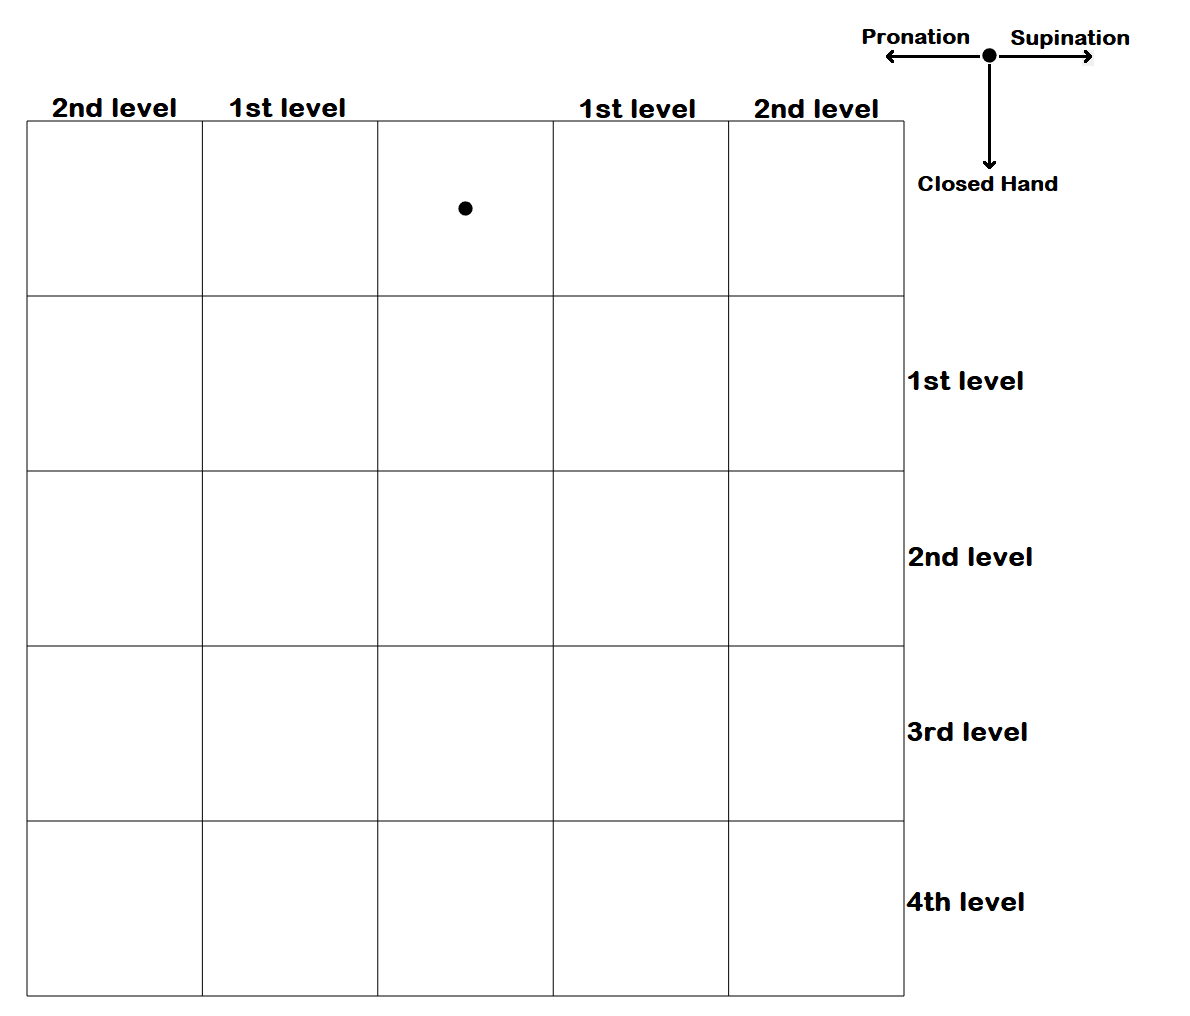
\includegraphics[width=0.45\textwidth]{figures/gridmap2}  
	\caption{Image of the grid map and cursor used in the experiment. Performing supination moved the cursor to the right, pronation moved it to the left and closing the hand moved it downwards. For left-handed subjects, the rotational movements were reversed. Opening the hand moved the cursor upwards, and was used as a correction movement if needed.}
	\label{fig:meth:gridmap} 
\end{figure}